\documentclass[journal,12pt,twocolumn]{IEEEtran}

\usepackage{setspace}
\usepackage{gensymb}

\singlespacing


\usepackage[cmex10]{amsmath}

\usepackage{amsthm}

\usepackage{mathrsfs}
\usepackage{txfonts}
\usepackage{stfloats}
\usepackage{bm}
\usepackage{cite}
\usepackage{cases}
\usepackage{subfig}

\usepackage{longtable}
\usepackage{multirow}

\usepackage{enumitem}
\usepackage{mathtools}
\usepackage{steinmetz}
\usepackage{tikz}
\usepackage{circuitikz}
\usepackage{verbatim}
\usepackage{tfrupee}
\usepackage[breaklinks=true]{hyperref}
\usepackage{graphicx}
\usepackage{tkz-euclide}

\usetikzlibrary{calc,math}
\usepackage{listings}
    \usepackage{color}                                            %%
    \usepackage{array}                                            %%
    \usepackage{longtable}                                        %%
    \usepackage{calc}                                             %%
    \usepackage{multirow}                                         %%
    \usepackage{hhline}                                           %%
    \usepackage{ifthen}                                           %%
    \usepackage{lscape}     
\usepackage{multicol}
\usepackage{chngcntr}

\DeclareMathOperator*{\Res}{Res}

\renewcommand\thesection{\arabic{section}}
\renewcommand\thesubsection{\thesection.\arabic{subsection}}
\renewcommand\thesubsubsection{\thesubsection.\arabic{subsubsection}}

\renewcommand\thesectiondis{\arabic{section}}
\renewcommand\thesubsectiondis{\thesectiondis.\arabic{subsection}}
\renewcommand\thesubsubsectiondis{\thesubsectiondis.\arabic{subsubsection}}


\hyphenation{op-tical net-works semi-conduc-tor}
\def\inputGnumericTable{}                                 %%

\lstset{
%language=C,
frame=single, 
breaklines=true,
columns=fullflexible
}
\begin{document}


\newtheorem{theorem}{Theorem}[section]
\newtheorem{problem}{Problem}
\newtheorem{proposition}{Proposition}[section]
\newtheorem{lemma}{Lemma}[section]
\newtheorem{corollary}[theorem]{Corollary}
\newtheorem{example}{Example}[section]
\newtheorem{definition}[problem]{Definition}

\newcommand{\BEQA}{\begin{eqnarray}}
\newcommand{\EEQA}{\end{eqnarray}}
\newcommand{\define}{\stackrel{\triangle}{=}}
\bibliographystyle{IEEEtran}

\providecommand{\mbf}{\mathbf}
\providecommand{\pr}[1]{\ensuremath{\Pr\left(#1\right)}}
\providecommand{\qfunc}[1]{\ensuremath{Q\left(#1\right)}}
\providecommand{\sbrak}[1]{\ensuremath{{}\left[#1\right]}}
\providecommand{\lsbrak}[1]{\ensuremath{{}\left[#1\right.}}
\providecommand{\rsbrak}[1]{\ensuremath{{}\left.#1\right]}}
\providecommand{\brak}[1]{\ensuremath{\left(#1\right)}}
\providecommand{\lbrak}[1]{\ensuremath{\left(#1\right.}}
\providecommand{\rbrak}[1]{\ensuremath{\left.#1\right)}}
\providecommand{\cbrak}[1]{\ensuremath{\left\{#1\right\}}}
\providecommand{\lcbrak}[1]{\ensuremath{\left\{#1\right.}}
\providecommand{\rcbrak}[1]{\ensuremath{\left.#1\right\}}}
\theoremstyle{remark}
\newtheorem{rem}{Remark}
\newcommand{\sgn}{\mathop{\mathrm{sgn}}}
\providecommand{\abs}[1]{\left\vert#1\right\vert}
\providecommand{\res}[1]{\Res\displaylimits_{#1}} 
\providecommand{\norm}[1]{\left\lVert#1\right\rVert}
%\providecommand{\norm}[1]{\lVert#1\rVert}
\providecommand{\mtx}[1]{\mathbf{#1}}
\providecommand{\mean}[1]{E\left[ #1 \right]}
\providecommand{\fourier}{\overset{\mathcal{F}}{ \rightleftharpoons}}
%\providecommand{\hilbert}{\overset{\mathcal{H}}{ \rightleftharpoons}}
\providecommand{\system}{\overset{\mathcal{H}}{ \longleftrightarrow}}
	%\newcommand{\solution}[2]{\textbf{Solution:}{#1}}
\newcommand{\solution}{\noindent \textbf{Solution: }}
\newcommand{\cosec}{\,\text{cosec}\,}
\providecommand{\dec}[2]{\ensuremath{\overset{#1}{\underset{#2}{\gtrless}}}}
\newcommand{\myvec}[1]{\ensuremath{\begin{pmatrix}#1\end{pmatrix}}}
\newcommand{\mydet}[1]{\ensuremath{\begin{vmatrix}#1\end{vmatrix}}}

\numberwithin{equation}{subsection}

\makeatletter
\@addtoreset{figure}{problem}
\makeatother
\let\StandardTheFigure\thefigure
\let\vec\mathbf

\renewcommand{\thefigure}{\theproblem}

\def\putbox#1#2#3{\makebox[0in][l]{\makebox[#1][l]{}\raisebox{\baselineskip}[0in][0in]{\raisebox{#2}[0in][0in]{#3}}}}
     \def\rightbox#1{\makebox[0in][r]{#1}}
     \def\centbox#1{\makebox[0in]{#1}}
     \def\topbox#1{\raisebox{-\baselineskip}[0in][0in]{#1}}
     \def\midbox#1{\raisebox{-0.5\baselineskip}[0in][0in]{#1}}
\vspace{3cm}
\title{Assignment 2}
\author{Sachinkumar Dubey}

\maketitle
\newpage

\bigskip
\renewcommand{\thefigure}{\theenumi}
\renewcommand{\thetable}{\theenumi}
Download all python codes from 
\begin{lstlisting}
https://github.com/sachinomdubey/Matrix-theory/Assignment2/codes
\end{lstlisting}
%
and latex-tikz codes from 
%
\begin{lstlisting}
https://github.com/sachinomdubey/Matrix-theory/Assignment2
\end{lstlisting}
%

\noindent Q no. 73. Find the angle between the following pair of lines:
\begin{enumerate}
\item
\begin{align}
L_1: \quad \vec{x} &= \myvec{2\\-5\\1} + \lambda_1\myvec{3 \\ 2 \\6}
\\
L_2: \quad \vec{x} &= \myvec{7\\-6\\0} + \lambda_2\myvec{1 \\ 2 \\2}
\end{align}
\item
\begin{align}
L_1: \quad \vec{x} &= \myvec{3\\1\\-2} + \lambda_1\myvec{1 \\ -1 \\-2}
\\
L_2: \quad \vec{x} &= \myvec{2\\-1\\-56} + \lambda_2\myvec{3 \\ -5 \\-4}
\end{align}
\end{enumerate}
%
\\
\solution 
\begin{enumerate}
\item The direction vectors of the lines are
\myvec{3 \\ 2 \\6} and \myvec{1 \\ 2 \\2}. \\
Thus, the angle $\theta$ between two vectors is given by 
%
\begin{align}
\label{eq:line_scalar_prod}
\cos \theta &= \frac{\vec{a}^T\vec{b}}{\norm{\vec{a}}\norm{\vec{b}}}
\\
&=\frac{19}{3\times7}
\\
\implies \theta &= 25.21\degree
\end{align}
\item The direction vectors of the lines are
\myvec{1 \\ -1 \\-2} and \myvec{3 \\ -5 \\-4}. \\
Thus, the angle $\theta$ between two vectors is given by 
%
\begin{align}
\label{eq:line_scalar_prod}
\cos \theta &= \frac{\vec{a}^T\vec{b}}{\norm{\vec{a}}\norm{\vec{b}}}
\\
&=\frac{16}{\sqrt6\times\sqrt50}
\\
\implies \theta &= 22.52\degree
\end{align}
\end{enumerate} 
\\
\textbf{Note :} In both problems, the respective pair of lines do not intersect each other (called skew lines), The obtained angle is the angle between the normal vectors of the lines. The proof that the pair of lines do not intersect is as follows:\\
\\
\textbf{Problem 1 :} Equating the x, y and z components of both lines, we get three equations as follow:
\begin{align}
2+3\lambda_1=7+\lambda_2 \\
-5+2\lambda_1=-6+2\lambda_2 \\
1+6\lambda_1=2\lambda_2
\end{align}
Solving the first two equations, 
\begin{align}
\lambda_1=\frac{11}{4} \\
\lambda_2=\frac{13}{4}
\end{align}
Substituting these values in the third equation, we find that it does not solve it. Hence, these three equations are inconsistent, which proves that the two lines do not intersect in the 3D plane.\\
\\ \newpage
\begin{figure}[h!]
\centering
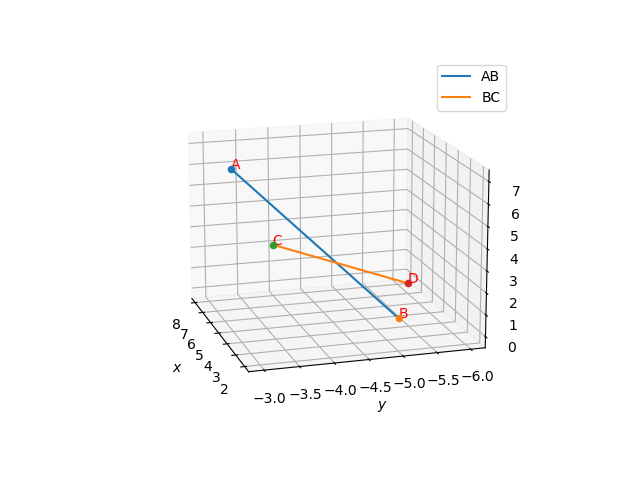
\includegraphics[width=10cm, height=8cm]{Figure_1}
\caption{Problem 1 : Lines crossing each other, but not intersecting}
\label{Fig2}
\end{figure}
\\
\textbf{Problem 2 :} Equating the x, y and z components of both lines, we get three equations as follow:
\begin{align}
3+\lambda_1=2+3\lambda_2 \\
1-\lambda_1=-1-5\lambda_2 \\
-2-2\lambda_1=-56-4\lambda_2
\end{align}
Solving the first two equations, 
\begin{align}
\lambda_1=\frac{-11}{2} \\
\lambda_2=\frac{-3}{2}
\end{align}
Substituting these values in the third equation, we find that it does not solve it. Hence, these three equations are inconsistent, which proves that the two lines do not intersect in the 3D plane.
\newpage
\begin{figure}[h!]
\centering
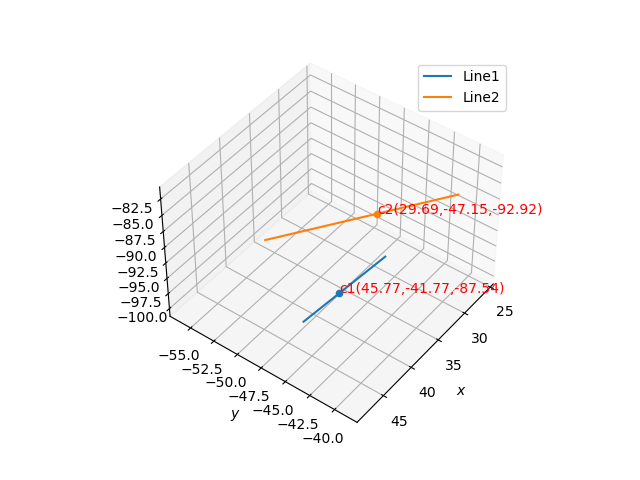
\includegraphics[width=10cm, height=8cm]{Figure_2}
\caption{Problem 2 : Lines crossing each other, but not intersecting}
\label{Fig2}
\end{figure}
\end{document}